\providecommand{\xrng}[1]{\X{#1}_{\mathcal{R}}}
\providecommand{\xnll}[1]{\X{#1}_{\mathcal{N}}}
\providecommand{\yrng}[1]{\Y{#1}_{\mathcal{R}}}
\providecommand{\ynll}[1]{\Y{#1}_{\mathcal{N}}}

\providecommand{\mat}[2] {\left[\begin{array}{#1}#2\end{array}\right]}
\providecommand{\rat}[2] {\mathbf{R}^{\mathrm{#2}}\paren{#1}}

\newcommand{\eps}{\epsilon}
\newcommand{\lam}{\lambda}

%% order
\providecommand{\order}[1] { \mathcal{o}\paren{#1} }
\providecommand{\Order}[1] { \mathcal{O}\paren{#1} }

\providecommand{\recip}[1] {\frac{1}{#1}}
\providecommand{\recipp}[1]{\paren{ \frac{1}{#1} }}
\providecommand{\half}     {\recip{2}}
	
%% matrix properties
\providecommand{\dim}[1]   {\text{dim}\paren{ #1 } }
\providecommand{\rank}[1]  {\text{rank}\paren{#1}}

\providecommand{\dist}[1]  {\text{dist}\paren{#1}}

%%%%%
\def\rot{\textbf{R}\paren{\theta}}

\def\TT      {\mathrm{T}}

\newcommand{\archetype} {\Aexample  = \Yshade \Sigmaexampleb \Xtshade}
\newcommand{\archetypez}{\Aexample &= \Yshade \Sigmaexampleb \Xtshade}

\newcommand{\pihalf} {\frac{\pi}{2}}


\newcommand{ \ls }  {\A{} x = b}
\newcommand{ \lsa } {\A{} x & = b }
\newcommand{ \zero }{\textbf{0}}
\newcommand{ \one } {\textbf{1}}
%\newcommand{ \pivot } {1 \negthickspace\negthickspace\negmedspace\bigcirc}
\newcommand{ \pivot } {\boxed{1}}
\definecolor{ltgray}{gray}{0.9}
\definecolor{veryltgray}{gray}{0.95}

\providecommand{\titlea}{$\A{}$ &=& $\Y{}$ & $\sig{}$ & $\X{T}$}
%\providecommand{\lgc}{\mat{c>{\columncolor{ltgray}}c>{\columncolor{ltgray}}c}}

%\newcommand{\fullpath}{\pathname"declarations"}

%%other definitions
\newcommand{\astar}[0] { \textbf{A\!}^{*} }

\providecommand{\A}[1] { \textbf{A}^{\mathrm{\!#1}} }
\providecommand{\B}[1] { \textbf{B}^{\mathrm{\!#1}} }
\providecommand{\C}[1] { \textbf{C}^{\mathrm{\!#1}} }
\providecommand{\D}[1] { \textbf{D}^{\mathrm{\!#1}} }
\providecommand{\LL}[1]{ \textbf{L}^{\mathrm{\!#1}} }
\providecommand{\M}[1] { \textbf{M}^{\mathrm{\!#1}} }
\providecommand{\N}[1] { \textbf{N}^{\mathrm{\!#1}} }
\providecommand{\pee}[1]{\textbf{P}^{\mathrm{\!#1}} }
\providecommand{\Q}[1] { \textbf{Q}^{\mathrm{\!#1}} }
\providecommand{\R}[1] { \textbf{R}^{\mathrm{\!#1}} }
\providecommand{\RR}[1]{ \textbf{R}\paren{#1} }
\providecommand{\T}[1] { \textbf{T}^{\mathrm{\!#1}} }
\providecommand{\V}[1] { \textbf{V}^{\mathrm{\!#1}} }
\providecommand{\U}[1] { \textbf{U}^{\mathrm{\!#1}} }
\providecommand{\X}[1] { \textbf{X}^{\mathrm{\!#1}} }
\providecommand{\Y}[1] { \textbf{Y}^{\mathrm{\!#1}} }
\providecommand{\Z}[1] { \textbf{Z}^{\mathrm{\!#1}} }
\providecommand{\ess}[1]{\textbf{S}^{\mathrm{\!#1}} }
\providecommand{\J}[2] { \textbf{J}^{\!#2}_{#1} }
\providecommand{\JJ}[1]{ \textbf{J}_{#1} }
\providecommand{\E}[1] { \textbf{E}_{#1} }
\providecommand{\G}[1] { \textbf{G}_{\mathrm{#1}} }
\providecommand{\I}[1] { \textbf{I}_{#1} }
\providecommand{\K}[1] { \textbf{K}_{#1} }
\providecommand{\W}[1] { \textbf{W}_{\mathrm{#1}} }
\providecommand{\sig}[1] { \Sigma^{\mathrm{#1}} }

\providecommand{\QR} { \Q{}\R{} }
\providecommand{\LU} { \L{}\U{} }
\providecommand{\CS} { \C{}\ess{} }


\endinput
\providecommand{\grafa} {\includegraphics[ width = 1in ]}
\providecommand{\grafb} {\includegraphics[ width = 1in ]}
\providecommand{\grafc} {\includegraphics[ width = 1in ]}
\providecommand{\grafd} {\includegraphics[ width = 1in ]}
\providecommand{\grafe} {\includegraphics[ width = 1in ]}




\endinput
\newcommand{\abs}[1]         {\left|#1\right|}
\providecommand{\norm}[1]    {\left\lVert#1\right\rVert}
\providecommand{\normo}[1]   {\left\lVert#1\right\rVert_{1}}
\providecommand{\normt}[1]   {\left\lVert#1\right\rVert_{2}}
\providecommand{\norminf}[1] {\left\lVert#1\right\rVert_\infty}
\providecommand{\normp}[1]   {\left\lVert#1\right\rVert_{p}}
\providecommand{\normf}[1]   {\left\lVert#1\right\rVert_F}

\providecommand{\norms}[1]   {\left\lVert#1\right\rVert^{2}}
\providecommand{\normos}[1]  {\left\lVert#1\right\rVert_{1}^{2}}
\providecommand{\normts}[1]  {\left\lVert#1\right\rVert_{2}^{2}}
\providecommand{\norminfs}[1]{\left\lVert#1\right\rVert_\infty^{2}}
\providecommand{\normps}[1]  {\left\lVert#1\right\rVert_{p}^{2}}
\providecommand{\normfs}[1]  {\left\lVert#1\right\rVert_F^{2}}

\endinput
\input{\fullpath/pauli}
\newcommand{ \cero }{
\textcolor[gray]{0.8}{0}
}
%%
%% vectors
%%
\newcommand{ \xhatt } {\left[
\begin{array}{c}
 1 \\
 0
\end{array}
\right]
}

\newcommand{ \yhatt } {\left[
\begin{array}{c}
  0 \\
  1
\end{array}
\right]
}

\newcommand{ \xhattt } {\left[
\begin{array}{c}
 1 \\
 0 \\
 0
\end{array}
\right]
}

\newcommand{ \yhattt } {\left[
\begin{array}{c}
  0 \\
  1 \\
  0
\end{array}
\right]
}

\newcommand{ \zhattt } {\left[
\begin{array}{c}
  0 \\
  0 \\
  1
\end{array}
\right]
}

\newcommand{ \xtwo } {\left[
\begin{array}{c}
 x \\
 y
\end{array}
\right]
}

\newcommand{ \xthree } {\left[
\begin{array}{c}
 x \\
 y \\
 z
\end{array}
\right]
}

%%
%% origins
%%
\newcommand{ \otwo }
{\mat{c}{0\\0}}

\newcommand{ \othree }
{\mat{c}{0\\0\\0}}

%%
%% matrices
%%
\newcommand{ \itwo } {
\mat{cc}{
 1 & 0 \\
 0 & 1 
}}

\newcommand{ \ithree } {
\mat{ccc}{
 1 & 0 & 0 \\
 0 & 1 & 0 \\
 0 & 0 & 1
}}

\newcommand{ \ifour } {
\mat{cccc}{
 1 & 0 & 0 & 0 \\
 0 & 1 & 0 & 0 \\
 0 & 0 & 1 & 0 \\
 0 & 0 & 0 & 1 \\
}}

\newcommand{ \ktwo } {
\mat{cc}{
 0 & 1 \\
 1 & 0 
}}

\newcommand{ \kthree } {
\mat{ccc}{
 0 & 0 & 1 \\
 0 & 1 & 0 \\
 1 & 0 & 0
}}

\newcommand{ \kfour } {
\mat{cccc}{
 0 & 0 & 0 & 1 \\
 0 & 0 & 1 & 0 \\
 0 & 1 & 0 & 0 \\
 1 & 0 & 0 & 0 \\
}}

% bys
\newcommand{\by}[2]      {#1 \times #2}
\newcommand{\byy}[1]     {#1 \times #1}
\newcommand{\bymn}[0]    {\by{m}{n}}
\newcommand{\bymm}[0]    {\byy{m}}
\newcommand{\bynn}[0]    {\byy{n}}
\newcommand{\bynm}[0]    {\by{n}{m}}
\newcommand{\bymr}[0]    {\by{m}{\rho}}
\newcommand{\byrn}[0]    {\by{\rho}{n}}

% vector spaces
\newcommand{\real}[1]    {\mathbb{R}^{#1}}
\newcommand{\cmplx}[1]   {\mathbb{C}^{#1}}
\newcommand{\either}[1]  {\cmplx{#1}}
\newcommand{\ir}[0]      {\in\real{}}
\newcommand{\ic}[0]      {\in\cmplx{}}
\newcommand{\icm}[0]     {\in\cmplxm}
\newcommand{\icn}[0]     {\in\cmplxn}
\newcommand{\icmn}[0]    {\in\cmplxmn}
\newcommand{\irmn}[0]    {\in\realmn}
\newcommand{\icmnr}[0]   {\in\cmplxmnr}
\newcommand{\ints}[0]    {\mathbb{Z}}
\newcommand{\natnum}[0]  {\mathbb{N}}

\newcommand{\iints}[0]   {\in \mathbb{Z}}
\newcommand{\inatnum}[0] {\in \mathbb{N}}

\newcommand{\realall}[3] {\real{\by{#1}{#2}}_{#3} }
\newcommand{\cmplxall}[3]{\cmplx{\by{#1}{#2}}_{#3} }

\newcommand{\realn}[0]   {\real{n}}
\newcommand{\realm}[0]   {\real{m}}
\newcommand{\realmn}[0]  {\real{\bymn}}
\newcommand{\realnn}[0]  {\real{\byy{n}}}
\newcommand{\realmm}[0]  {\real{\byy{m}}}
\newcommand{\realmmr}[0] {\real{\byy{m}}_{\rho}}
\newcommand{\realmmm}[0] {\realmm_{m}}

\newcommand{\cmplxn}[0]  {\cmplx{n}}
\newcommand{\cmplxm}[0]  {\cmplx{m}}
\newcommand{\cmplxnn}[0] {\cmplx{\byy{n}}}
\newcommand{\cmplxmm}[0] {\cmplx{\byy{m}}}
\newcommand{\cmplxmn}[0] {\cmplx{\bymn}}
\newcommand{\cmplxmr}[0] {\cmplx{\bymr}}
\newcommand{\cmplxrn}[0] {\cmplx{\byrn}}
\newcommand{\cmplxmnr}[0]{\cmplx{\bymn}_{\rho}}
\newcommand{\cmplxmmm}[0]{\cmplxmm_{m}}
\newcommand{\cmplxmnm}[0]{\cmplxmn_{m}}
\newcommand{\cmplxnnr}[0]{\cmplxnn_{\rho}}
\newcommand{\cmplxmnn}[0]{\cmplxmn_{n}}

% spans
\newcommand{\spn}[1]     {\text{sp\,} \lst{ #1 }}


\endinput  %  -  -  -  -  -  -  -  -  -  -  -  -  -  -  -  -  -  -  -  -
\providecommand{\tildx}{\tilde{x}}
\providecommand{\tildy}{\tilde{y}}
\providecommand{\tildz}{\tilde{z}}

\providecommand{\hatx}{\hat{x}}
\providecommand{\haty}{\hat{y}}
\providecommand{\hatz}{\hat{z}}

\newcommand{\rhohat}{\hat{\rho}}

\endinput
\providecommand{\ngti}  {\quad \xrightarrow[n\to\infty]{} \quad}
\providecommand{\qlraq} {\quad \longrightarrow \quad}
\providecommand{\qLraq} {\quad \Longrightarrow \quad}
\providecommand{\qiff}  {\quad \iff \quad}

\providecommand{\arrnz} {\xrightarrow[\nti]{}}

\endinput
\newcommand{ \svdl }{singular value decomposition}
\newcommand{ \svdp }{singular value decomposition (SVD)}
\newcommand{ \ft }{Fundamental Theorem}
\newcommand{ \ftola }{\ft \ of Linear Algebra}
\newcommand{ \qr }{$\QR$ decomposition}

\providecommand{\mm}{{\it Mathematica}}
\providecommand{\ml}{Octave}

\endinput
\providecommand{\svd}[1]    { \Y{}\, \sig{}   \, \X{ \mathrm{#1} } }
\providecommand{\svdt}[1]   { \X{}\, \sig{T}  \, \Y{ \mathrm{#1} } }
\providecommand{\svdd}[1]   { \Y{\mathrm{#1}}\A{}\X{} }
\providecommand{\mpgi}[1]   { \X{}\, \sig{(+)}\, \Y{ \mathrm{#1} } }
\providecommand{\svdthin}[1]{ \widetilde{\Y{}}\, \widetilde{\sig{}}\, \widetilde{\mathbf{X}}^{\mathrm{#1}} }

\newcommand{\xrng}[1]{\X{#1}_{\mathcal{R}}}
\newcommand{\xnll}[1]{\X{#1}_{\mathcal{N}}}
\newcommand{\yrng}[1]{\Y{#1}_{\mathcal{R}}}
\newcommand{\ynll}[1]{\Y{#1}_{\mathcal{N}}}

\newcommand{\yrn}[1]  { \mat{c>{\columncolor{ltgray}}c}{\yrng{} & \ynll{#1}} }
\newcommand{\ytrn}[1] { \mat{c}{\yrng{#1} \\ \rowcolor{ltgray} \ynll{}}}

\newcommand{\xrn}[1]  { \mat{c>{\columncolor{ltgray}}c}{\xrng{#1} & \xnll{}}}
\newcommand{\xtrn}[1] { \mat{c}{\xrng{#1} \\ \rowcolor{ltgray} \xnll{}}}

\newcommand{\yft}[1]  { \mat{c>{\columncolor{ltgray}}c}{\rnga{} & \nlla{#1}} }
\newcommand{\xft}[1]  { \mat{c>{\columncolor{ltgray}}c}{\rnga{#1} & \nlla{}} }

\newcommand{\ytft}[1] { \mat{c}{\rnga{}   \\ \rowcolor{ltgray}\nlla{#1}} }
\newcommand{\xtft}[1] { \mat{c}{\rnga{#1} \\ \rowcolor{ltgray}\nlla{}} }

\providecommand{\svda}[1]  {\A{}   & = \svd{#1}}
\providecommand{\svdta}[1] {\A{#1} & = \svdt{#1}}

\providecommand{\svdax}[1] {\A{}     = \svd{#1}}
\providecommand{\svdtax}[1]{\A{#1}   = \svdt{#1}}

\providecommand{\mpgia}[1] {\Ap    & = \mpgi{#1}}
\providecommand{\mpgiax}[1]{\Ap      = \mpgi{#1}}

\providecommand{\svdtag}[1]{\Y{}_{ #1 }\, \Sigma_{ #1 }\, \X{*}_{ #1 }}
\providecommand{\svdtagA}[1]{\A{}_{ #1 } = \svdtag{#1}}


\endinput
\section{Vectors}
\label{sec:vectors}
Row vectors are fun targets for the \svdl. It's very easy to visualize the domain and codomain.

%%
\subsection{\vv s}
Consider the \vv \ below:
\begin{equation}
  v=\mat{c}{1\\\frac{1}{2}}.
  \label{eq:cases:2v}
\end{equation}
Hopefully the rank of the system is obvious:
\begin{equation}
  \rho = \min\lst{m,n}= \min\lst{2,1} = 1
\end{equation}

The decomposition will have these form factors
\begin{equation}
  \begin{array}{ccccc}
  \A{} &=& \Y{} & \sig{} & \X{T}\\
  \by{m}{n}&=&\paren{\by{m}{m}}&\paren{\by{m}{n}}&\paren{\by{n}{n}}\\
  \by{2}{1}&=&\paren{\by{2}{2}}&\paren{\by{2}{1}}&\paren{\by{1}{1}},
  \end{array}
\end{equation}
as depicted below:
\begin{figure}[htbp] %  figure placement: here, top, bottom, or page
   \centering
   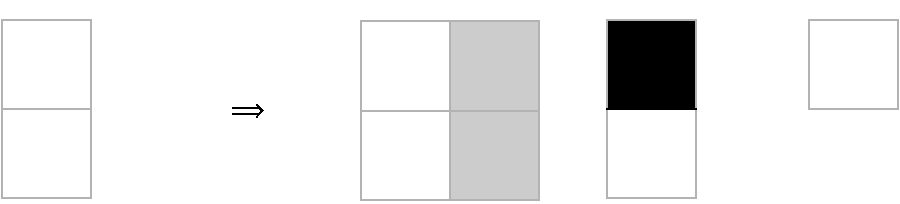
\includegraphics[ width = 4in ]{pdf/more_examples/svd_02_01_01} 
%  ` \caption{example caption}
   \label{fig:examples:21}
\end{figure}

The $\X{}$ matrix is trivial. Since it must be unitary the magnitude is one:
\begin{equation}
  \X{}= \mat{c}{1}.
\end{equation}
The lone singular value is the scale factor $r=\sqrt{2^{2}+\frac{1}{2}^{2}}$ which is the length of the vector:
\begin{equation}
  \sig{} = \mat{c}{\frac{\sqrt{5}}{2}\\0}.
\end{equation}
  For the codomain matrix we start with the image and normalize the column vector:
\begin{equation}
  \Y{}=\mat{cc}{c_{1}&c_{2}}, \qquad c_{1}=\frac{\sqrt{5}}{2}\mat{c}{2\\1}.
\end{equation}
The only quantity missing now is the null space vector $c_{2}$. Pick an orthogonal complement to $c_{1}$ and the codomain basis matrix is
\begin{equation}
  \Y{}=\frac{1}{\sqrt{5}}\mat{rr}{2&1\\1&-2}.
\end{equation}
The \svdl \ is then
\begin{equation}
  \begin{split}
    \svda{T}\\
    \mat{c}{1\\\frac{1}{2}} &= \frac{1}{\sqrt{5}}
    \mat{rr}{2&-1\\1&2}
    \mat{c}{\frac{\sqrt{5}}{2}\\0}
    \mat{c}{1}.
  \end{split}
  \label{eq:cases:2vdecomp}
\end{equation}

%%
\subsection{\vvv s}
Consider this \vvv:
\begin{equation}
  v = \mat{r}{1\\2\\-2}.
\end{equation}
The decomposition will have the shapes given by this
\begin{equation}
  \begin{array}{ccccc}
  \A{} &=& \Y{} & \sig{} & \X{T}\\
  \by{m}{n}&=&\paren{\by{m}{m}}&\paren{\by{m}{n}}&\paren{\by{n}{n}}\\
  \by{3}{1}&=&\paren{\by{3}{1}}&\paren{\by{3}{1}}&\paren{\by{1}{1}},
  \end{array}
\end{equation}
as shown here:
\begin{figure}[htbp] %  figure placement: here, top, bottom, or page
   \centering
   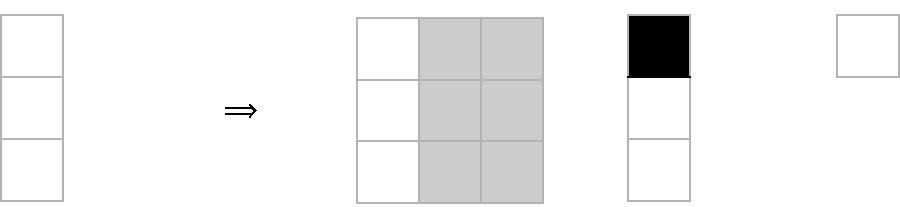
\includegraphics[ width = 4in ]{pdf/more_examples/svd_03_01_01} 
%   \caption{example caption}
   \label{fig:examples:31}
\end{figure}

We can use this vector to seed the codomain matrix:
\begin{equation}
  \Y{}_{*,1} = \frac{1}{3}\mat{r}{1\\2\\-2}.
\end{equation}
This leaves the null space vectors. A first candidate is 
\begin{equation}
  \Y{}_{*,2} = \frac{1}{\sqrt{2}}\mat{r}{0\\1\\1}.
\end{equation}
Using an inspection-based algorithm we can pick a vector like
\begin{equation}
  \Y{}_{*,3} = \frac{1}{\sqrt{18}}\mat{r}{4\\-1\\1}.
\end{equation}
The lone singular value is the length of the vector. The \svdl \ becomes
\begin{equation}
  \begin{split}
    \svda{T}\\
    \mat{r}{1\\2\\-2} &=
    \left[
\begin{array}{ r >{\columncolor{ltgray}}r >{\columncolor{ltgray}}r }
  \frac{1}{3} & 0 & \frac{4}{ \sqrt{18} } \\[5pt]
  \frac{2}{3} & \frac{1}{\sqrt{2}} & -\frac{1}{ \sqrt{18} } \\[5pt]
 -\frac{2}{3} & \frac{1}{\sqrt{2}} &  \frac{1}{ \sqrt{18} }
\end{array}
\right] 
    \left[
\begin{array}{c}
 3 \\ \hline
 0 \\
 0
\end{array}
\right]
  \mat{c}{1}.
  \end{split}
\end{equation}

The shortcut won't work. 
\begin{equation}
  v = \mat{c}{\sin\theta \\ 0 \\ \cos\theta}.
\end{equation}

\begin{equation}
  \begin{split}
    \W{y} = v v^{\mathrm{T}} &= \mat{c}{\sin\theta \\ 0 \\ \cos\theta}\mat{ccc}{\sin\theta & 0 & \cos\theta}\\
    &= \mat{ccc}{\sin^{2}\theta & 0 & \sin\theta \cos\theta\\ 0 & 0 & 0 \\ \sin\theta \cos\theta & 0 & \cos^{2}\theta}
  \end{split}
\end{equation}


Characteristic polynomial
Use cofactor expansion to compute the determinant
\begin{equation}
  \begin{split}
    p(\lambda) &= \det \paren{\W{y} - \lambda \I{3}}\\ &= 
    \det\mat{c|r|c}{\sin^{2}\theta - \lambda & 0 & \sin\theta \cos\theta\\\hline 0 & - \lambda & 0 \\ \sin\theta \cos\theta & 0 & \cos^{2}\theta- \lambda} \\
    &= \paren{\sin^{2}\theta - \lambda}\det\mat{cc}{-\lambda & 0 \\ 0 & \cos^{2}\theta- \lambda}\\ & \quad- 0 \det\mat{cc}{0 & 0 \\ \sin\theta \cos\theta & \cos^{2}\theta- \lambda}\\
     & \quad + \paren{\cos^{2}\theta - \lambda}\det\mat{cc}{0 & -\lambda \\ \sin\theta \cos\theta & 0}\\
  \end{split}
\end{equation}

The roots of the characteristic polynomial are the eigenvalues
\begin{equation}
  p(\lambda) = \lambda^{2}\paren{\lambda-1} = 0
\end{equation}
leads to the spectrum
\begin{equation}
  \lambda\paren{\W{y}} = \lst{1,0,0}.
\end{equation}
Therefore there is one singular value, 
\begin{equation}
  \sigma_{1} = 1.
\end{equation}
The eigenvector solves
\begin{equation}
  \begin{split}
    \W{y}u &= \lambda u\\
    \mat{ccc}{\sin^{2}\theta & 0 & \sin\theta \cos\theta\\ 0 & 0 & 0 \\ \sin\theta \cos\theta & 0 & \cos^{2}\theta} \mat{c}{u_{1} \\ 0 \\ u_{3}} & = \mat{c}{u_{1} \\ 0 \\ u_{3}}
  \end{split}
\end{equation}
This reduces to the system
\begin{equation}
\mat{cc}
{\sin^{2}\theta & \sin\theta \cos\theta\\
 \sin\theta \cos\theta & \cos^{2}\theta}
\mat{c}{u_{1} \\ u_{3}} = \mat{c}{u_{1} \\ u_{3}}
\end{equation}



%%
\subsection{$10-$vectors}
You can quickly verify that
\begin{equation}
  \begin{split}
    \svda{T}\\
    \mat{r}{1\\0\\0\\0\\0\\0\\0\\0\\0\\0} &=
    \left[
\begin{array}{ r >{\columncolor{ltgray}}r >{\columncolor{ltgray}}r >{\columncolor{ltgray}}r >{\columncolor{ltgray}}r >{\columncolor{ltgray}}r >{\columncolor{ltgray}}r >{\columncolor{ltgray}}r >{\columncolor{ltgray}}r >{\columncolor{ltgray}}r }
  1 & 0 & 0 & 0 & 0 & 0 & 0 & 0 & 0 & 0 \\
  0 & 1 & 0 & 0 & 0 & 0 & 0 & 0 & 0 & 0 \\
  0 & 0 & 1 & 0 & 0 & 0 & 0 & 0 & 0 & 0 \\
  0 & 0 & 0 & 1 & 0 & 0 & 0 & 0 & 0 & 0 \\
  0 & 0 & 0 & 0 & 1 & 0 & 0 & 0 & 0 & 0 \\
  0 & 0 & 0 & 0 & 0 & 1 & 0 & 0 & 0 & 0 \\
  0 & 0 & 0 & 0 & 0 & 0 & 1 & 0 & 0 & 0 \\
  0 & 0 & 0 & 0 & 0 & 0 & 0 & 1 & 0 & 0 \\
  0 & 0 & 0 & 0 & 0 & 0 & 0 & 0 & 1 & 0 \\
  0 & 0 & 0 & 0 & 0 & 0 & 0 & 0 & 0 & 1 \\
\end{array}
\right] 
    \left[
\begin{array}{c}
 1 \\ \hline
 0 \\
 0 \\
 0 \\
 0 \\
 0 \\
 0 \\
 0 \\
 0 \\
 0
\end{array}
\right]
  \mat{c}{1}.
  \end{split}
\end{equation}

This is such a simple exercise because the column vectors are already unit vectors.

A Givens rotation by an angle $\theta$ in the $4-8$ plane does not affect the decomposition because the codomain matrix $\Y{}$ is still orthogonal
\begin{equation}
  \Y{'} = 
      \left[
\begin{array}{ c >{\columncolor{ltgray}}c >{\columncolor{ltgray}}c >{\columncolor{ltgray}}c >{\columncolor{ltgray}}c >{\columncolor{ltgray}}c >{\columncolor{ltgray}}c >{\columncolor{ltgray}}c >{\columncolor{ltgray}}c >{\columncolor{ltgray}}c }
  1 & 0 & 0 & 0 & 0 & 0 & 0 & 0 & 0 & 0 \\
  0 & 1 & 0 & 0 & 0 & 0 & 0 & 0 & 0 & 0 \\
  0 & 0 & 1 & 0 & 0 & 0 & 0 & 0 & 0 & 0 \\
  0 & 0 & 0 & \cos \theta & 0 & 0 & 0 & -\sin \theta & 0 & 0 \\
  0 & 0 & 0 & 0 & 1 & 0 & 0 & 0 & 0 & 0 \\
  0 & 0 & 0 & 0 & 0 & 1 & 0 & 0 & 0 & 0 \\
  0 & 0 & 0 & 0 & 0 & 0 & 1 & 0 & 0 & 0 \\
  0 & 0 & 0 & \sin \theta & 0 & 0 & 0 & \cos \theta & 0 & 0 \\
  0 & 0 & 0 & 0 & 0 & 0 & 0 & 0 & 1 & 0 \\
  0 & 0 & 0 & 0 & 0 & 0 & 0 & 0 & 0 & 1 \\
\end{array}
\right] 
\end{equation}

Yet another rotation 1-9:
\begin{equation}
  \Y{'} = 
      \left[
\begin{array}{ c >{\columncolor{ltgray}}c >{\columncolor{ltgray}}c >{\columncolor{ltgray}}c >{\columncolor{ltgray}}c >{\columncolor{ltgray}}c >{\columncolor{ltgray}}c >{\columncolor{ltgray}}c >{\columncolor{ltgray}}c >{\columncolor{ltgray}}c }
  \cos \phi & 0 & 0 & 0 & 0 & 0 & 0 & 0 & -\sin \phi & 0 \\
  0 & 1 & 0 & 0 & 0 & 0 & 0 & 0 & 0 & 0 \\
  0 & 0 & 1 & 0 & 0 & 0 & 0 & 0 & 0 & 0 \\
  0 & 0 & 0 & \cos \theta & 0 & 0 & 0 & -\sin \theta & 0 & 0 \\
  0 & 0 & 0 & 0 & 1 & 0 & 0 & 0 & 0 & 0 \\
  0 & 0 & 0 & 0 & 0 & 1 & 0 & 0 & 0 & 0 \\
  0 & 0 & 0 & 0 & 0 & 0 & 1 & 0 & 0 & 0 \\
  0 & 0 & 0 & \sin \theta & 0 & 0 & 0 & \cos \theta & 0 & 0 \\
  \sin \phi & 0 & 0 & 0 & 0 & 0 & 0 & 0 & \cos \phi & 0 \\
  0 & 0 & 0 & 0 & 0 & 0 & 0 & 0 & 0 & 1 \\
\end{array}
\right] 
\end{equation}


\endinput
% The 8 Gell-Mann matrices for SU(3)
\newcommand{ \gma } {
\mat{ccc}{
 0 & 1 & 0 \\
 1 & 0 & 0 \\
 0 & 0 & 0
}}
\newcommand{ \gmb } {
\mat{crc}{
 0 & -i & 0 \\
 i & 0 & 0 \\
 0 & 0 & 0
}}
\newcommand{ \gmc } {
\mat{crc}{
 1 & 0 & 0 \\
 0 & -1 & 0 \\
 0 & 0 & 0
}}
\newcommand{ \gmd } {
\mat{ccc}{
 0 & 0 & 1 \\
 0 & 0 & 0 \\
 1 & 0 & 0
}}\newcommand{ \gme } {
\mat{ccr}{
 0 & 0 & -i \\
 0 & 0 & 0 \\
 i & 0 & 0
}}\newcommand{ \gmf } {
\mat{ccc}{
 0 & 0 & 0 \\
 0 & 0 & 1 \\
 0 & 1 & 0
}}\newcommand{ \gmg } {
\mat{ccr}{
 0 & 0 & 0 \\
 0 & 0 & -i \\
 0 & i & 0
}}\newcommand{ \gmh } {
\sthree
\mat{ccr}{
 1 & 0 & 0 \\
 0 & 1 & 0 \\
 0 & 0 & -2
}
}
\def\psymbol {+}
\def\pssymbol{(\psymbol)}
\def\Ap      {\A{\psymbol}}
\def\leftinv {\Ap\A{}}
\def\rightinv{\A{}\Ap}
\def\AinvL   {\A{-\mathrm{L}}}
\def\AinvR   {\A{-\mathrm{R}}}
\def\AinvB   {\A{-\mathrm{L,R}}}
\def\mpcone  {\A{}\Ap\A{}}
\def\mpctwo  {\Ap\A{}\Ap}


\endinput
%% Example matrices

\newcommand{ \Aexample }
{
    \mat{ rr }
      {
       1 & -1 \\
      -1 &  1 \\
       1 & -1
      }
}

\newcommand{ \Aplus }
{
  \frac{1}{6}
  \mat{rrr}
  {
   1 &  \phantom{-}1 &  1\\
  -1 &  1 & -1
  }
}

\newcommand{ \Atexample } 
{
    \mat{ rrr }
      {
       1 & -1 & 1 \\
      -1 & 1 & -1 \\
      }
}

\newcommand{\phivector}
{
  \mat{c}
  {
  2\\1\\0
  }
}

\newcommand{\ximatrix}
{
  \mat{c}
  {
  \xi \\ \eta
  }
}

\newcommand{ \Sigmatexamplea } {
\left[
\begin{array}{c|cc}
 \sqrt{6} & 0 & 0 \\ \hline
 0 & 0 & 0
\end{array}
\right]
}

\newcommand{ \Sigmaexampleb } {
\left[
\begin{array}{c|c}
 \sqrt{6} & 0 \\ \hline
 0 & 0 \\
 0 & 0
\end{array}
\right]
}

\newcommand{ \Sigmaexample } {
\left[
\begin{array}{cc}
 \sqrt{6} & 0 \\ 
 0 & 0 \\
 0 & 0
\end{array}
\right]
}

\newcommand{ \Sigmainverse } {
\left[
\begin{array}{c|cc}
 \ssix & 0 & 0 \\[5pt] \hline
 0 & 0 & 0
\end{array}
\right]
}

\newcommand{ \Xshadex } {
\left[
\begin{array}{ r >{\columncolor{ltgray}}r }
  \stwo & \stwo \\[5pt]
 -\stwo & \phantom{-}\stwo
\end{array}
\right]
}

\newcommand{ \Xshade } {
\stwo
\left[
\begin{array}{ r >{\columncolor{ltgray}}r }
  1 & 1 \\
 -1 & \phantom{-}1
\end{array}
\right]
}

\newcommand{ \Xtshade } {
\stwo
\left[
\begin{array}{ rr }
  1 & -1 \\[5pt]
\rowcolor{ltgray}
  \phantom{-}1 &  1
\end{array}
\right]
}

\newcommand{ \Yshade } {
\left[
\begin{array}{ r >{\columncolor{ltgray}}c >{\columncolor{ltgray}}r }
  \sthree & 0 & -\frac{2}{ \sqrt{6} } \\[5pt]
 -\sthree & \stwo &  \ssix \\[5pt]
  \sthree & \stwo & -\ssix
\end{array}
\right] 
}

\newcommand{ \Ytshade } {
\left[
\begin{array}{ rrr }
  \sthree & -\sthree & \sthree \\[5pt]
\rowcolor{ltgray}
   0 & \stwo &  \stwo \\[5pt]
\rowcolor{ltgray}
  -\frac{2}{ \sqrt{6} } & \ssix & -\ssix
\end{array}
\right] 
}

\newcommand{ \veca } {
\mat{r}{0\\1\\1}
}

\newcommand{ \vecb } {
\mat{r}{-2\\-1\\1}
}

\newcommand{ \Xexample } {
\stwo
\left[
\begin{array}{ rr }
   1 & 1 \\[5pt]
  -1 & \phantom{-}1
\end{array}
\right]
}


\newcommand{ \Xtexample } {
\stwo
\left[
\begin{array}{ rr }
  \phantom{-}1 & -1 \\[5pt]
  1 &  1
\end{array}
\right]
}

\newcommand{ \Sigmatexample } {
\left[
\begin{array}{ccc}
 \sqrt{6} & 0 & 0 \\ \hline
 0 & 0 & 0
\end{array}
\right]
}

\newcommand{ \Aexamplecol } {
\left[
\begin{array}{ r|r }
  1 & -1 \\
 -1 & 1 \\
  1 & -1
\end{array}
\right]
}


\newcommand{ \Aexamplerow } {
\left[
\begin{array}{ rr }
 1 & -1 \\ \hline
 -1 & 1 \\ \hline
 1 & -1
\end{array}
\right]
}

\newcommand{ \Aexamplepi } {
  \frac{1}{6}
  \mat{rrr}
  { 1 & -1 &  1\\
   -1 &  1 & -1
  }
}

%%
%% ch 01 exercises
\providecommand{\locala}{\sqrt{\frac{1}{130} \paren{65 + \sqrt{65}}}}  % cos
\providecommand{\localb}{\sqrt{\frac{1}{130} \paren{65 - \sqrt{65}}}}  % sin

\providecommand{\localc}{\sqrt{\half - \frac{7}{2 \sqrt{65}}}}  % cos
\providecommand{\locald}{\sqrt{\half + \frac{7}{2 \sqrt{65}}}}  % sin

\newcommand{\ncases}{$n=3,5,10,25,50,100$}

\newcommand{\cgray}{>{\columncolor{ltgray}}}

\endinput
\newtheorem{thm} {Theorem}
\newtheorem{cor} {Corollary}
\newtheorem{lem} {Lemma}
\newtheorem{defn}{Definition}

\endinput
%% common fractions
\newcommand{\rtwo}  { \frac{1}{2} }
\newcommand{\rthree}{ \frac{1}{3} }
\newcommand{\rfour} { \frac{1}{4} }
\newcommand{\rfive} { \frac{1}{5} }
\newcommand{\rsix}  { \frac{1}{6} }

\newcommand{\stwo}  { \frac{1}{\sqrt{2}} }
\newcommand{\sthree}{ \frac{1}{\sqrt{3}} }
\newcommand{\sfive} { \frac{1}{\sqrt{5}} }
\newcommand{\ssix}  { \frac{1}{\sqrt{6}} }

\newcommand{\nstwo}  { \frac{-1}{\sqrt{2}} }
\newcommand{\nsthree}{ \frac{-1}{\sqrt{3}} }
\newcommand{\nsfive} { \frac{-1}{\sqrt{5}} }
\newcommand{\nssix}  { \frac{-1}{\sqrt{6}} }

\endinput
\numberwithin{section}{chapter}
\numberwithin{equation}{chapter}
\numberwithin{figure}{chapter}
\numberwithin{table}{chapter}


\endinput
\providecommand{\Ain}[1] {\A{\by{m}{n}}_{#1}}
\providecommand{\Ar} [1] {\A{}\in\real {\by{#1}{#1}}}
\providecommand{\Arr}[2] {\A{}\in\real {\by{#1}{#2}}}
\providecommand{\Arrr}[3]{\A{}\in\real {\by{#1}{#2}}_{#3}}
\providecommand{\Ac} [1] {\A{}\in\cmplx{\by{#1}{#1}}}
\providecommand{\Acc}[2] {\A{}\in\cmplx{\by{#1}{#2}}}
\providecommand{\Accc}[3]{\A{}\in\cmplx{\by{#1}{#2}}_{#3}}
\providecommand{\Accmn}  {\Acc{m}{n}}
\providecommand{\Arrmn}  {\Arr{m}{n}}
\providecommand{\Amnr}   {\Accmn_{\rho}}
\providecommand{\Amnrr}  {\Arrmn_{\rho}}

\providecommand{\by}[2]  {#1 \times #2}
\providecommand{\bys}[1] {#1 \times #1}
\providecommand{\byy}[1] {#1 \times #1}
\providecommand{\byt}[2] {\mathit{#1} \times \mathit{#2}}
\providecommand{\bymn}   {\by{m}{n}}
\providecommand{\bymm}   {\bys{m}}
\providecommand{\bynn}   {\bys{n}}

\providecommand{\realmn} {\real{\by{m}{n}}}
\providecommand{\realmm} {\real{\byy{m}}}
\providecommand{\realnn} {\real{\byy{n}{n}}}

\providecommand{\realm} {\real{m}}
\providecommand{\realn} {\real{n}}

\providecommand{\cmplxmn} {\cmplx{\by{m}{n}}}
\providecommand{\cmplxmm} {\cmplx{\byy{m}}}
\providecommand{\cmplxnn} {\cmplx{\byy{n}{n}}}

\providecommand{\cmplxm} {\cmplx{m}}
\providecommand{\cmplxn} {\cmplx{n}}


\endinput

% fundamental projectors
\def\projra {\mathbf{P}_{\rng{\A{}}}}
\def\projrap{\mathbf{P}_{\rng{\A{}}^{\perp}}}
\def\projna {\mathbf{P}_{\nll{\A{}}}}
\def\projnap{\mathbf{P}_{\nll{\A{}}^{\perp}}}

\def\projrat {\mathbf{P}_{\rng{\A{T}}}}
\def\projratp{\mathbf{P}_{\rng{\A{T}}^{\perp}}}
\def\projnat {\mathbf{P}_{\nll{\A{T}}}}
\def\projnatp{\mathbf{P}_{\nll{\A{T}}^{\perp}}}

\providecommand{\aap}[1]   {\Y{}\,\sig{}\,\sig{(+)}\,\Y{#1}}
\providecommand{\apa}[1]   {\X{}\,\sig{(+)}\,\sig{}\,\X{#1}}

%\providecommand{\pra}[1]   {\Y{}\,\J{m}{\rho}\Y{#1}}
%\providecommand{\pnap}[1]  {\X{}\,\J{n}{\rho}\,\X{#1}}

\providecommand{\pra}[1]   {\yrng{}\yrng{#1}}
\providecommand{\pnap}[1]  {\xrng{}\xrng{#1}}

\endinput
\providecommand{\paren}[1] { \left(  #1 \right) }
\providecommand{\inner}[1] { \langle #1 \rangle }
\providecommand{\brac}[1]  { \left[  #1 \right] }
\providecommand{\lst}[1]   { \left\{ #1 \right\} }

\endinput
%% 2 x 2 x 2 example matrix

\newcommand{ \matrixalpha }
{
    \mat{ rc }
      {
       1 & 2 \\
      -1 & 2
      }
}

\newcommand{ \matrixalphat }
{
    \mat{ cr }
      {
       1 & -1 \\
       2 &  2
      }
}

\newcommand{ \matrixalphapi }
{
    \frac{1}{4}
    \mat{ cr }
      {
       2 & -2 \\
       1 &  1
      }
}

\newcommand{ \matrixalphaY }
{
    \stwo
    \mat{ cr }
      {
       1 &  1 \\
       1 & -1
      }
}

\newcommand{ \matrixalphaYt }
{
    \stwo
    \mat{ cr }
      {
       1 &  1 \\
       1 & -1
      }
}

\newcommand{ \matrixalphaX }
{
    \ktwo
}

\newcommand{ \matrixalphaXt }
{
    \ktwo
}

\newcommand{ \matrixalphasigma }
{
    \sqrt{2}
    \mat{ cc }
      {
       2 & 0 \\
       0 & 1
      }
}

\newcommand{ \matrixalphasigmat }
{
    \matrixalphasigma
}

\newcommand{ \matrixalphasigmapi }
{
    \stwo
    \mat{ cc }
      {
       \rtwo & 0 \\
       0 & 1
      }
}

%% 3 x 2 x 2 example matrix

\newcommand{ \matrixbravo }
{
    \mat{ ccc }
      {
       0 & 3 & 0 \\
       1 & 2 & 2
      }
}

\newcommand{ \matrixbravot }
{
    \mat{ cc }
      {
       0 & 1 \\
       3 & 2 \\
       0 & 2 
      }
}

\newcommand{ \matrixbravopi }
{
    \frac{1}{15}
    \mat{ rc }
      {
      -2 & 3 \\
       5 & 0 \\
      -4 & 6 
      }
}

\newcommand{ \matrixbravoY }
{
    \stwo
    \mat{ cr }
      {
       1 & -1 \\
       1 &  1
      }
}

\newcommand{ \matrixbravoYt }
{
    \stwo
    \mat{ rc }
      {
       1 & 1 \\
      -1 & 1
      }
}

\newcommand{ \matrixbravoX }
{
    \mat{ cc>{\columncolor{ltgray}}c }
      {
       \frac{1}{\sqrt{30}} & \frac{1} {\sqrt{6}} & \frac{-2}{\sqrt{5}} \\
       \frac{5}{\sqrt{30}} & \frac{-1}{\sqrt{6}} & 0 \\
       \frac{2}{\sqrt{30}} & \frac{2} {\sqrt{6}} & \frac{1}{\sqrt{5}} \\
      }
}

\newcommand{ \matrixbravoXt }
{
    \mat{ ccc }
      {
       \frac{1}{\sqrt{30}} & \frac{5}{\sqrt{30}} & \frac{2}{\sqrt{30}} \\
       \frac{1}{\sqrt{6}}  & \frac{-1}{\sqrt{6}} & \frac{2}{\sqrt{6}} \\
       \rowcolor{ltgray}
       \frac{-2}{\sqrt{5}} & 0                   & \frac{1}{\sqrt{5}} \\
      }
}

\newcommand{ \matrixbravosigma }
{
    \mat{ cc|c }
      {
       \sqrt{15} & 0 & 0 \\
       0         & \sqrt{3} & 0
      }
}

\newcommand{ \matrixbravosigmat }
{
    \mat{ cc }
      {
       \sqrt{15} & 0 \\
       0         & \sqrt{3} \\ \hline
       0         & 0 
      }
}

\newcommand{ \matrixbravosigmapi }
{
    \mat{ cc }
      {
       \frac{1}{\sqrt{15}} & 0 \\
       0         & \frac{1}{\sqrt{3}} \\[5pt] \hline
       0         & 0 
      }
}

\newcommand{ \matrixbravoApA }
{
    \rfive
    \mat{ ccc }
      {
       1 & 0 & 2 \\
       0 & 5 & 0 \\
       2 & 0 & 4
      }
}

\newcommand{ \matrixbravoAAp }
{
    \itwo
}
	
\providecommand{\td}[2]  {\frac{d#1}{d#2}}
\providecommand{\tdd}[2] {\frac{d^{2}#1}{d#2^{2}}}
\providecommand{\tdn}[3] {\frac{d^{#3}#1}{d#2^{#3}}}
\providecommand{\tdt}[1] {\frac{d#1}{dt}}
\providecommand{\tdx}[1] {\frac{d#1}{dx}}
\providecommand{\pd}[2]  {\frac{\partial#1}{\partial#2}}
\providecommand{\pdt}[2] {\frac{\partial#1}{\partial t}}
\providecommand{\pdx}[2] {\frac{\partial#1}{\partial x}}
\providecommand{\pdd}[2] {\frac{\partial^{2}#1}{\partial#2^{2}}}
\providecommand{\pdn}[3] {\frac{\partial^{#3}#1}{\partial#2^{#3}}}

\newcommand{\intunit}[1] {\int_{0}^{1}{#1 \, dx}}

\endinput
%% jtwo, jthree, jfour, jfive

%% jonejtwo, \kjonejtwo, \kjtwojone, jtwojone, jtwojtwo, kjtwojtwo

\newcommand{ \jtwo }
{
    \mat{ cc }
      {
       1     & 1 \\
       \cero & 1 \\
      }
}

\newcommand{ \jthree }
{
    \mat{ ccc }
      {
       1     & 1     & \cero \\
       \cero & 1     & 1 \\
       \cero & \cero & 1
      }
}

\newcommand{ \jfour }
{
    \mat{ cccc }
      {
       1     & 1     & \cero & \cero \\
       \cero & 1     & 1     & \cero \\
       \cero & \cero & 1     & 1 \\
       \cero & \cero & \cero & 1 \\
      }
}

\newcommand{ \jfive }
{
    \mat{ ccccc }
      {
       1 & 1 & 0 & 0 & 0 \\
       0 & 1 & 1 & 0 & 0 \\
       0 & 0 & 1 & 1 & 0 \\
       0 & 0 & 0 & 1 & 1 \\
       0 & 0 & 0 & 0 & 1 \\
      }
}

\newcommand{ \jonejtwo }
{
    \mat{ c|cc }
      {
       1 & 0 & 0 \\
       0 & 1 & 1 \\\hline
       0 & 0 & 1
      }
}

\newcommand{ \jtwojone }
{
    \mat{ cc|c }
      {
       1 & 1 & 0 \\
       0 & 1 & 0 \\\hline
       0 & 0 & 1
      }
}

\newcommand{ \kjonejtwo }
{
    \mat{ cc|c }
      {
       0 & 0 & 1 \\\hline
       1 & 1 & 0 \\
       0 & 1 & 0
      }
}

\newcommand{ \kjtwojone }
{
    \mat{ c|cc }
      {
       0 & 1 & 1 \\
       0 & 0 & 1 \\\hline
       1 & 0 & 0
      }
}
\newcommand{ \jtwojtwo }
{
    \mat{ cc|cc }
      {
       1 & 1 & 0 & 0 \\
       0 & 1 & 0 & 0 \\\hline
       0 & 0 & 1 & 1 \\
       0 & 0 & 0 & 1 \\
      }
}

\newcommand{ \kjtwojtwo }
{
    \mat{ cc|cc }
      {
       0 & 0 & 1 & 1 \\
       0 & 0 & 0 & 1 \\\hline
       1 & 1 & 0 & 0 \\
       0 & 1 & 0 & 0 \\
      }
}
	
\def\tr{\text{tr}}
\def\spn {span}
\def\sgn {\text{sgn }}
%\def\span{span}
\def\mx{max}
\def\dm{dim}
\def\adj{adj}
\def\Arg{Arg}
\def\rref{rref}
\def\ns{null space}

\endinput
\providecommand{\prdm}[1]  {\A{ \mathrm{#1} }\A{}}
\providecommand{\prdmm}[1] {\A{}\,\A{ \mathrm{#1} }}

\providecommand{\prdmx}[1] {\A{ \mathrm{#1} }\A{}}
\providecommand{\prdmy}[1] {\A{}\,\A{ \mathrm{#1} }}

\providecommand{\invx}     {\Ap\A{}}
\providecommand{\invy}     {\A{}\,\Ap}

\providecommand{\vx}[1]    {\X{}\,\sig{\pssymbol}\,\sig{}\,\X{#1}}
\providecommand{\vy}[1]    {\Y{}\,\sig{}\,\sig{\pssymbol}\,\Y{#1}}

\providecommand{\wx}[1]    {\X{}\,\sig{T}\,\sig{}\,\X{#1}}
\providecommand{\wy}[1]    {\Y{}\,\sig{}\,\sig{T}\,\Y{#1}}

\providecommand{\sx}       {\sig{T}\,\sig{}}
\providecommand{\sy}       {\sig{} \,\sig{T}}

\providecommand{\tx}       {\sig{\pssymbol}\,\sig{}}
\providecommand{\ty}       {\sig{} \,\sig{\pssymbol}}

\providecommand{\prodx}[2] {\X{}_{#2}\,\X{#1}_{#2}}
\providecommand{\prody}[2] {\Y{}_{#2}\,\Y{#1}_{#2}}


\endinput